\documentclass{article}
\usepackage{tikz}
 
\title{}

\begin{document}

\maketitle
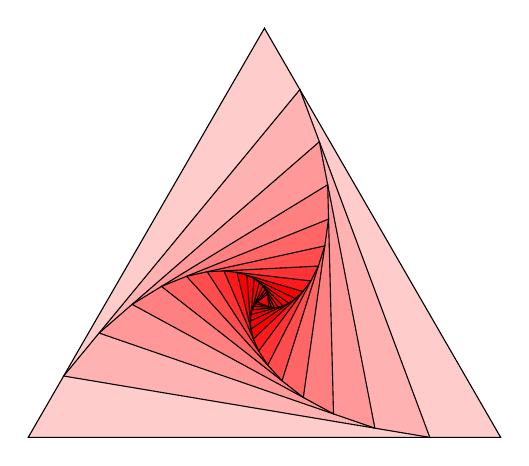
\begin{tikzpicture}
\newcounter{density}
\setcounter{density}{20}
    \def\couleur{red}
    \path[coordinate] (0,0)  coordinate(A)
                ++( 60:6cm) coordinate(B)
                ++(-60:6cm) coordinate(C);
    \draw[fill=\couleur!\thedensity] (A) -- (B) -- (C) -- cycle;
    \foreach \x in {1,...,15}{%
        \pgfmathsetcounter{density}{\thedensity+10}
        \setcounter{density}{\thedensity}
        \path[coordinate] coordinate(X) at (A){};
        \path[coordinate] (A) -- (B) coordinate[pos=.15](A)
                            -- (C) coordinate[pos=.15](B)
                            -- (X) coordinate[pos=.15](C);
        \draw[fill=\couleur!\thedensity] (A)--(B)--(C)--cycle;
    }
\end{tikzpicture}

\end {document}